\section{Beweis des Fünffarbensatzes}
\authors{Anna Siess und Vincent Meise }
\begin{satz} \label{Satz}
Jeder planare Graph ist mit fünf Farben färbbar, sodass keine zwei benachbarte Knoten mit der gleichen Farbe gefärbt sind.
\end{satz}
Das Problem, einen Graphen mit möglichst wenig Farben zu färben, sodass jeder Knoten anders als all seinen Nachbarknoten gefärbt ist, beschäftigt die Menschen schon lange. Bei planaren Graphen gibt es tatsächlich eine obere Schranke: Nur vier Farben genügen. Dies ist allerdings sehr schwer zu beweisen. Im Folgenden soll daher bewiesen werden, warum man einen planaren Graphen mit nur fünf Farben färben kann.\\
Ansätze zur Beweisführung:\\
Für den Beweis wird das Prinzip der Induktion, sowie folgendes Korollar \ref{minimalgrad} benutzt: $\delta \leq 5$.\\
\subsection{Ansatz: Schluss vom Allgemeinen auf Konkretes}
Im ersten Ansatz wird versucht den Satz zu beweisen, indem zuerst bewiesen wird, dass der Satz \ref{Satz} für alle Graphen gilt, für die Lemma \ref{lemma1} $|E|\leq3|V|-6$ gilt, und anschließend auf planare Graphen geschlossen wird.
Dafür gibt es allerdings ein Gegenbeispiel, welches diesen Ansatz widerlegt.\\
\begin{figure}
\centering
	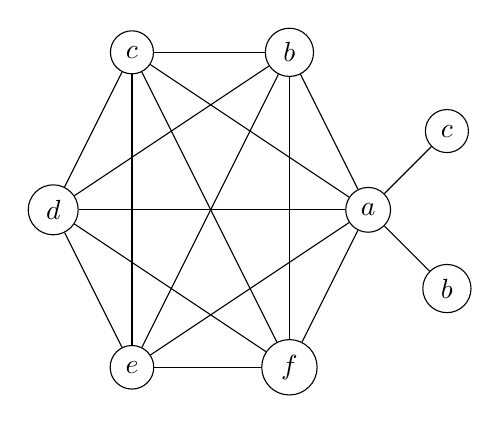
\begin{tikzpicture}
	\node[circle,draw](1) at (4,2){$a$};
	\node[circle,draw](2) at (3,4){$b$};
	\node[circle,draw](3) at (1,4){$c$};
	\node[circle,draw](4) at (0,2){$d$};
	\node[circle,draw](5) at (1,0){$e$};
	\node[circle,draw](6) at (3,0){$f$};
	\node[circle,draw](7) at (5,1){$b$};
	\node[circle,draw](8) at (5,3){$c$};
	\draw (1)--(2);
	\draw (1)--(3);
	\draw (1)--(4);
	\draw (1)--(5);
	\draw (1)--(6);
	\draw (1)--(7);
	\draw (1)--(8);
	\draw (2)--(3);
	\draw (2)--(4);
	\draw (2)--(5);
	\draw (2)--(6);
	\draw (3)--(4);
	\draw (3)--(5);
	\draw (3)--(6);
	\draw (4)--(5);
	\draw (4)--(6);
	\draw (5)--(6);
	\end{tikzpicture}
	\caption{Gegenbeispiel zum Ansatz}
	\label{graph1}
\end{figure}
Wie man an dem Beispiel in Abbildung \ref{graph1} sieht, gibt es auch nicht-planare Graphen, die Lemma \ref{lemma1} gilt, aber es nicht ausreicht, nur fünf Farben zum Färben zu benutzen. Das liegt daran, dass sechs der acht Knoten untereinander allesamt verbunden sind. Daher muss dieser Ansatz zur Findung eines Beweises aufgegeben werden.
\subsection{Ansatz: Umfärben der Knoten}\begin{proof}
Die Grundidee ist, mit einem Worst-Case-Szenario durch Induktion zu zeigen, dass bei einem bereits korrekt gefärbten Graphen ein Knoten entfernt wird und ein neuer Knoten $v$ eingebunden werden kann, sodass der neue Knoten $v$ ebenfalls korrekt gefärbt werden kann. Dies soll durch Umfärben der Knoten möglich gemacht werden. Es werden unterschiedliche Fälle betrachtet, die durch das Lemma \ref{minimalgrad} begrenzt werden.\\
Es kann der Fall auftreten, dass der Knoten einen Grad kleiner fünf hat und somit das Einfärben kein Problem ist, da es immer eine Farbe gibt, in der $v$ gefärbt werden kann, ohne dass eine Farbe einer seiner Nachbarknoten benutzt wird.
\\Ein weiterer Fall ist, dass Knoten $v$ einen Grad fünf hat, aber die Nachbarknoten so eingefärbt sind, dass für diese nicht alle Farben verwendet werden. Knoten $v$ kann also in einer Farbe gefärbt werden, die nicht für die Nachbarknoten benutzt worden ist.
\\Der letzte Fall ist, dass Knoten $v$ Grad fünf hat und alle fünf Farben für die Nachbarknoten benutzt worden sind. Dies ist der letzte Fall, der 
Für den Beweis dieses Falles wird das oben erläuterte Lemma \ref{minimalgrad} benutzen, das es uns ermöglichen soll, ein Worst-Case-Szenario zu erstellen, da fünf die höchste Zahl ist, die laut Lemma \ref{lemma1}in Frage kommt.
Hierfür wird der erstmal farblose Knoten $v$ mit der Kantenanzahl 5 untersucht, der mit fünf weiteren Knoten verbunden ist, die paarweise unterschiedlich gefärbt sind -- also in insgesamt fünf unterschiedlichen Farben.\\
\begin{figure}
\centering
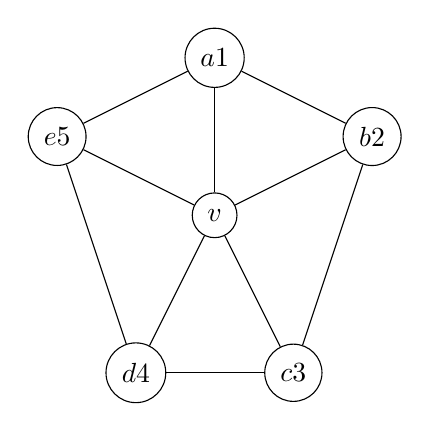
\begin{tikzpicture}
\node[circle,draw](1) at (2,5){$a1$};
\node[circle,draw](2) at (4,4){$b2$};
\node[circle,draw](3) at (3,1){$c3$};
\node[circle,draw](4) at (1,1){$d4$};
\node[circle,draw](5) at (0,4){$e5$};
\node[circle,draw](6) at (2,3){$v$};
\draw (1)--(2);
\draw (1)--(5);
\draw (1)--(6);
\draw (2)--(3);
\draw (2)--(6);
\draw (3)--(4);
\draw (3)--(6);
\draw (4)--(5);
\draw (4)--(6);
\draw (5)--(6);
\end{tikzpicture}
\caption{Färbungsproblem für Knoten v}
\label{graph2}
\end{figure}
Wegen dieser Situation ist es nicht möglich, Knoten $v$ direkt eine Farbe zuzuteilen. Mit diesem durch Korollar \ref{minimalgrad} erstellte Worst-Case-Szenario soll gezeigt werden, warum es immer möglich ist, einen Knoten $v$ korrekt zu färben, sodasser mit keinem benachbartem Knoten die gleiche Farbe hatund auch allle andere benachbarte Knoten nicht die gleiche Farbe haben.\\
Da alle fünf Farben zum Färben der Nachbarknoten bereits verwendet worden sind, wie man in Abbildung \ref{graph2} sehen kann, kann Knoten $v$ nicht sofort gefärbt werden. Daher wird der Ansatz verwendet, einige Knoten umzufärben, um so für Knoten $v$ eine Farbe zu erhalten, mit der es möglich ist, diesen problemlos einzufärben.\\
Wird nun $a$ von 1 auf 3, eine Farbe eines Knotens, der mit $v$ verbunden ist aber nicht mit $a$, umgefärbt, kann Knoten $v$ die Farbe 1 annehmen. Das wird in Abbildung \ref{graph3} dargestellt.
Ist Knoten $a$ mit einem Knoten weiteren der Farbe 3 verbunden, so muss dieser andere Knoten von 3 auf 1 umgefärbt werden. Folgt auf $a$ eine ganze Kette aus Knoten, die alle ausschließlich abwechselnd 1 und 3 gefärbt sind und mit Knoten $a$ benachbart sind, so müssen die Knoten mit Farbe 1 auf Farbe 3 umgefärbt werden und umgekehrt. So wird erreicht, dass trotz des Umfärbens alle bereits vorhandenen und gefärbten Knoten korrekt gefärbt sind. Im Folgenden wird ein solcher Kantenzug Umfärbungskantenzug genannt werden.\\
\begin{figure}
\centering
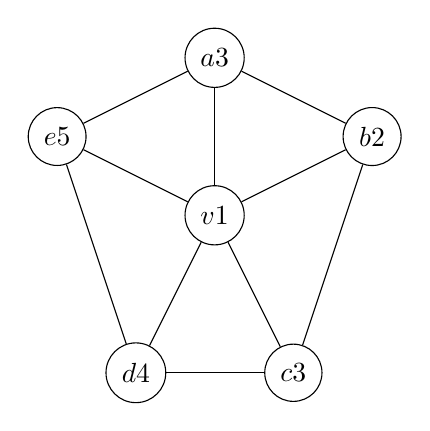
\begin{tikzpicture}
\node[circle,draw](1) at (2,5){$a3$};
\node[circle,draw](2) at (4,4){$b2$};
\node[circle,draw](3) at (3,1){$c3$};
\node[circle,draw](4) at (1,1){$d4$};
\node[circle,draw](5) at (0,4){$e5$};
\node[circle,draw](6) at (2,3){$v1$};
\draw (1)--(2);
\draw (1)--(5);
\draw (1)--(6);
\draw (2)--(3);
\draw (2)--(6);
\draw (3)--(4);
\draw (3)--(6);
\draw (4)--(5);
\draw (4)--(6);
\draw (5)--(6);
\end{tikzpicture}
\caption{Gewünschte Lösung des Problems}
\label{graph3}
\end{figure}
Nun wird eine Fallunterscheidung vorgenommen.\\
Im ersten Fall ist Knoten $a$ durch einen oben genannten Umfärbungskantenzug mit Knoten $c$ verbunden und somit wird Knoten $c$ von Farbe 3 auf Farbe 1 umgefärbt. Dadurch hat Knoten $v$ allerdings dieselbe Farbe wie Knoten $c$ und die Bedingung, dass zwei miteinander verbundene Knoten nicht mit der gleichen Farbe gefärbt sein dürfen, wäre nicht erfüllt. Dies wird in Abbildung \ref{graph4} gezeigt. Es muss also eine andere Möglichkeit gefunden werden, Knoten $v$ korrekt zu färben. Hierfür wird erst einmal die durch die Kette aus mit den Farben 1 und 3 gefärbten Knoten von Knoten $a$ zu Knoten $c$ gegeben Situation untersucht.\\
\begin{figure}
\centering
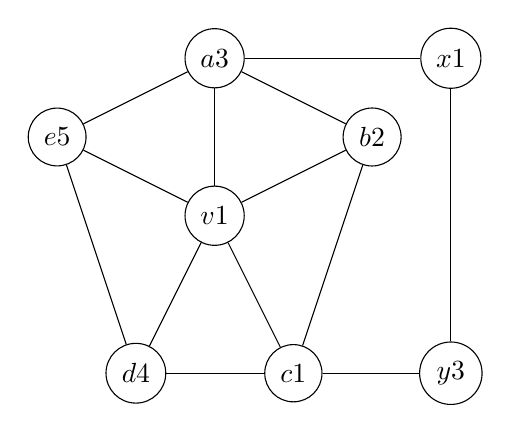
\begin{tikzpicture}
\node[circle,draw](7) at (7,5){$a3$};
\node[circle,draw](8) at (9,4){$b2$};
\node[circle,draw](9) at (8,1){$c1$};
\node[circle,draw](10) at (6,1){$d4$};
\node[circle,draw](11) at (5,4){$e5$};
\node[circle,draw](12) at (7,3){$v1$};
\node[circle,draw](13) at (10,5){$x1$};
\node[circle,draw](14) at (10,1){$y3$};
\draw (7)--(8);
\draw (7)--(11);
\draw (7)--(12);
\draw (8)--(9);
\draw (8)--(12);
\draw (9)--(10);
\draw (9)--(12);
\draw (10)--(11);
\draw (10)--(12);
\draw (11)--(12);
\draw (7)--(13);
\draw (13)--(14);
\draw (14)--(9);
\end{tikzpicture}
\caption{Problem durch Umfärbung}
\label{graph4}
\end{figure}
Durch den beliebig langen Umfärbungskantenzug aus nur Knoten mit Farben 1 und 3 wird der Knoten $b$ mit der Farbe 2, sowie die eventuell mit ihm verbundenen Knoten isoliert.\\
Knoten $b$ wird mit Farbe 4 umgefärbt. Wieder gilt, dass alle Knoten, die von Knoten $b$ aus über einen ausschließlich abwechselnd aus Knoten mit Farbe 2 und aus Farbe 4 bestehende Kantezug erreichbar sind, von Farbe 2 auf Farbe 4 umgefärbt werden und umgekehrt. Jeder solch Kantenzug von Knoten $b$ aus kann aufgrund des Umfärbungskantenzuges von $a$ nach $c$ nicht mit $d$ oder $e$ verbunden sein.\\
Somit kann für Knoten $v$ problemlos die Farbe 2 benutzt werden, wie man in Abbildung \ref{graph5} sehen kann.
\\
\begin{figure}
\centering
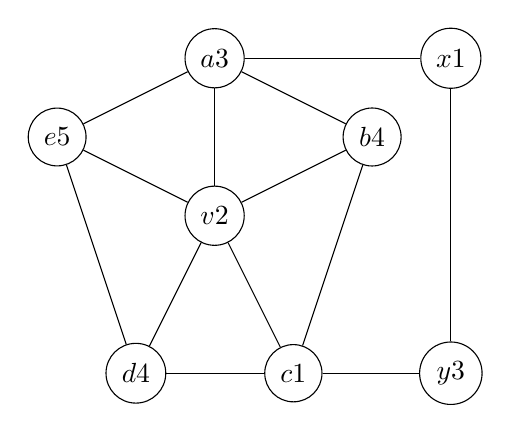
\begin{tikzpicture}
\node[circle,draw](7) at (7,5){$a3$};
\node[circle,draw](8) at (9,4){$b4$};
\node[circle,draw](9) at (8,1){$c1$};
\node[circle,draw](10) at (6,1){$d4$};
\node[circle,draw](11) at (5,4){$e5$};
\node[circle,draw](12) at (7,3){$v2$};
\node[circle,draw](13) at (10,5){$x1$};
\node[circle,draw](14) at (10,1){$y3$};
\draw (7)--(8);
\draw (7)--(11);
\draw (7)--(12);
\draw (8)--(9);
\draw (8)--(12);
\draw (9)--(10);
\draw (9)--(12);
\draw (10)--(11);
\draw (10)--(12);
\draw (11)--(12);
\draw (7)--(13);
\draw (13)--(14);
\draw (14)--(9);
\end{tikzpicture}
\caption{Neues Umfärben ohne Probleme}
\label{graph5}
\end{figure}
Im zweiten Fall ist Knoten $a$ nicht durch einen Umfärbungskantenzug mit Knoten $c$ verbunden und somit hat Knoten $v$ die Farbe 1 $a$, ohne dass weitere Umfärbungen notwendig sind. Wieder gilt, dass alle Knoten, die über einen Kantenzug aus abwechselnd Knoten mit Farbe 1 oder 3 mit $a$ verbunden sind, von 1 auf 3 umgefärbt werden und umgekehrt. Knoten $v$ hat somit eine Möglichkeit der Färbung, nämlich Farbe 1.\\
Durch das Beweisen dieses Worst-Case-Szenario kann bewiesen werden, dass der Satz \ref{Satz} für alle planare Graphen gilt, da jedes mal nicht nur Knoten $v$ betrachtet wird, sondern automatisch der gesamte Graph, der gegebenenfalls durch Umgefärbungen angepasst wird. Zudem wire durch die Umfärbungskantenzügen sichergestellt, dass keine neue problematische Knoten entstehen.\\

\end{proof}